\documentclass{beamer}

\newcommand{\course}{CS 1331 Introduction to Object Oriented Programming}
\newcommand{\lesson}{ArrayList and Swing}
\newcommand{\code}{http://www.cc.gatech.edu/~simpkins/teaching/gatech/cs1331/code}

\author[Chris Simpkins] 
{Christopher Simpkins \\\texttt{chris.simpkins@gatech.edu}}
\institute[Georgia Tech] % (optional, but mostly needed)

\date[CS 1331]{}

\subject{\lesson}


% If you have a file called "university-logo-filename.xxx", where xxx
% is a graphic format that can be processed by latex or pdflatex,
% resp., then you can add a logo as follows:

% \pgfdeclareimage[width=0.6in]{coc-logo}{cc_2012_logo}
% \logo{\pgfuseimage{coc-logo}}

\mode<presentation>
{
  \usetheme{Berlin}
  \useoutertheme{infolines}

  % or ...

 \setbeamercovered{transparent}
  % or whatever (possibly just delete it)
}

\usepackage{hyperref}
\usepackage{fancybox}
\usepackage{listings}
\usepackage[abbr]{harvard}

\usepackage[english]{babel}
% or whatever

\usepackage[utf8]{inputenc}
% or whatever

\usepackage{times}
\usepackage[T1]{fontenc}
% Or whatever. Note that the encoding and the font should match. If T1
% does not look nice, try deleting the line with the fontenc.


\usepackage{listings}
 
% "define" Scala
\lstdefinelanguage{scala}{
  morekeywords={abstract,case,catch,class,def,%
    do,else,extends,false,final,finally,%
    for,if,implicit,import,match,mixin,%
    new,null,object,override,package,%
    private,protected,requires,return,sealed,%
    super,this,throw,trait,true,try,%
    type,val,var,while,with,yield},
  otherkeywords={=>,<-,<\%,<:,>:,\#,@},
  sensitive=true,
  morecomment=[l]{//},
  morecomment=[n]{/*}{*/},
  morestring=[b]",
  morestring=[b]',
  morestring=[b]""",
}

\usepackage{color}
\definecolor{dkgreen}{rgb}{0,0.6,0}
\definecolor{gray}{rgb}{0.5,0.5,0.5}
\definecolor{mauve}{rgb}{0.58,0,0.82}
 
% Default settings for code listings
\lstset{frame=tb,
  language=scala,
  aboveskip=2mm,
  belowskip=2mm,
  showstringspaces=false,
  columns=flexible,
  basicstyle={\scriptsize\ttfamily},
  numbers=none,
  numberstyle=\tiny\color{gray},
  keywordstyle=\color{blue},
  commentstyle=\color{dkgreen},
  stringstyle=\color{mauve},
  frame=single,
  breaklines=true,
  breakatwhitespace=true,
  keepspaces=true
  %tabsize=3
}


\title[\course] % (optional, use only with long
                                      % paper titles)
{\lesson}

\subtitle{}
%% {Include Only If Paper Has a Subtitle}

\newcommand{\link}[2]{\href{#1}{\textcolor{blue}{\underline{#2}}}}


% If you wish to uncover everything in a step-wise fashion, uncomment
% the following command: 

% \beamerdefaultoverlayspecification{<+->}


\begin{document}

\begin{frame}
  \titlepage
\end{frame}


%------------------------------------------------------------------------
\begin{frame}[fragile]{Java Collections}

\begin{center}
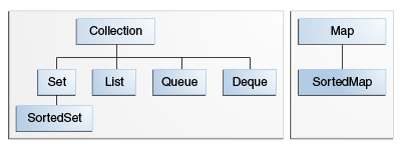
\includegraphics[width=4in]{colls-coreInterfaces.png}
\end{center}

{\tt ArralyList} and {\tt LinkedList} are the two basic {\tt List} implementations provided in the Java standard library.  The concepts we'll learn for {\tt ArrayList} apply to all of Java's collection classes.

\end{frame}
%------------------------------------------------------------------------

%------------------------------------------------------------------------
\begin{frame}[fragile]{{\tt ArrayList} Basics}


Create an {\tt ArrayList} with operator {\tt new}:
\begin{lstlisting}[language=Java]
  ArrayList tasks = new ArrayList();
\end{lstlisting}
Add items with {\tt add()}:
\begin{lstlisting}[language=Java]
  tasks.add("Eat");
  tasks.add("Sleep");
  tasks.add("Code");
\end{lstlisting}
Traverse with for-each loop:
\begin{lstlisting}[language=Java]
  for (Object task: tasks) {
      System.out.println(task);
  }
\end{lstlisting}

Note that the for-each loop implicitly uses an iterator.

\end{frame}
%------------------------------------------------------------------------

%------------------------------------------------------------------------
\begin{frame}[fragile]{Using Generics}


Supply a type argument in the angle brackets.  Read {\tt ArrayList<String>} as ``ArrayList of String''
\begin{lstlisting}[language=Java]
  ArrayList<String> strings = new ArrayList<String>();
  strings.add("Helluva"); strings.add("Engineer!");
\end{lstlisting}
If we try to add an object that isn't a {\tt String}, we get a compile error:
\begin{lstlisting}[language=Java]
  Integer BULL_DOG = Integer.MIN_VALUE;
  strings.add(BULL_DOG); // Won't compile
\end{lstlisting}

With a typed collection, we get autoboxing on insertion {\it and} retrieval:

\begin{lstlisting}[language=Java]
  ArrayList<Integer> ints = new ArrayList<>();
  ints.add(42);
  int num = ints.get(0);
\end{lstlisting}
Notice that we didn't need to supply the type parameter in the creation expression above.  Java inferred the type parameter from the declaration. (Note: this only works in Java 7 and above.)

See \link{\code/ArrayListGenericsDemo.java}{ArrayListGenericsDemo.java} for more.

\end{frame}
%------------------------------------------------------------------------

%------------------------------------------------------------------------
\begin{frame}[fragile]{The {\tt equals} Method and Collections}



\begin{itemize}
\item A class whose instances will be stored in a collection must have a properly implemented {\tt equals} method.
\item The {\tt contains} method in collections uses the {\tt equals} method in the stored objects.
\item The default implementation of {\tt equals} (object identity - true only for same object in memory) only rarely gives correct results.
\item Note that {\tt hashcode()} also has a defualt implementation that uses the object's memory address.  As a rule, whenever you override {\tt equals}, you should also override {\tt hashcode}
\end{itemize}


\end{frame}
%------------------------------------------------------------------------



%------------------------------------------------------------------------
\begin{frame}[fragile]{Swing}


Lots of stuff in Swing.  A few highlights:
\begin{itemize}
\item Container classes, e.g. {\tt JFrame} and {\tt JPanel}
\item Layout managers, e.g. {\tt FlowLayout}, {\tt BorderLayout}, {\tt GridLayout}
\item {\tt JLabel}s
\item {\tt Graphics} and drawing
\item Components with {\tt ActionListener}s, like {\tt JButton}
\begin{itemize}
\item Use {\tt private} inner classes
\item Avoid using a single monolithic class that extends JFrame or JPanel and implements ActionListener
\end{itemize}
\end{itemize}


\end{frame}
%------------------------------------------------------------------------

%------------------------------------------------------------------------
\begin{frame}[fragile]{The Wrong Way to Write an {\tt ActionListener}}


\begin{lstlisting}[language=Java,escapechar=`]
public class BadListener extends JFrame `\colorbox{yellow}{implements ActionListener}` {

    public BadListener() {
        super("Bad");
        setDefaultCloseOperation(EXIT_ON_CLOSE);
        JButton helloButton = new JButton("Hello");
        helloButton.addActionListener(this);
        JButton goodByeButton = new JButton("Good bye");
        goodByeButton.addActionListener(this);
        add(helloButton, BorderLayout.NORTH);
        add(goodByeButton, BorderLayout.SOUTH);
    }

    public void actionPerformed(ActionEvent e) {
        String button = `\colorbox{yellow}{e.getActionCommand()}`;
        if (button.equals("Hello")) {
            System.out.println("Hello was perssed.");
        } else if (button.equals("Good bye")) {
            System.out.println("Good bye was perssed.");
        }
    }
}
\end{lstlisting}

\end{frame}
%------------------------------------------------------------------------

%------------------------------------------------------------------------
\begin{frame}[fragile]{A Better Way to Write an {\tt ActionListener}}

\vspace{-.1in}
\begin{lstlisting}[language=Java]
public class BetterListener extends JFrame {

    private class HelloListener implements ActionListener {
        public void actionPerformed(ActionEvent e) {
            System.out.println("Hello was pressed.");
        }
    }
    private class GoodByeListener implements ActionListener {
        public void actionPerformed(ActionEvent e) {
            System.out.println("Good bye was pressed.");
        }
    }
    public BetterListener() {
        super("Better Listener");
        setDefaultCloseOperation(EXIT_ON_CLOSE);
        JButton helloButton = new JButton("Hello");
        helloButton.addActionListener(new HelloListener());
        JButton goodByeButton = new JButton("Good bye");
        goodByeButton.addActionListener(new GoodByeListener());
        add(helloButton, BorderLayout.NORTH);
        add(goodByeButton, BorderLayout.SOUTH);
    }
}
\end{lstlisting}


\end{frame}
%------------------------------------------------------------------------

% %------------------------------------------------------------------------
% \begin{frame}[fragile]{}


% \begin{lstlisting}[language=Java]

% \end{lstlisting}

% \begin{itemize}
% \item
% \end{itemize}


% \end{frame}
% %------------------------------------------------------------------------


\end{document}
